\subsection{Definição dos modelos genéricos}
Com base no INI-C (2018) e no levantamento das edificações de escritório de Vitória, foram 
propostos dois tipos de modelos genéricos como base para o estudo das modificações de 
otimização e de produção de energia. Estes modelos representam os dois cenários de ambiente 
construído mais observados na cidade de Vitória. Estes cenários são formados por edificações 
mais baixas, com 8 pavimentos, e as mais altas, com 19 pavimentos. As dimensões utilizadas 
como referência para a construção dos modelos genéricos foram resultado dos valores médios 
observados nas edificações que compõe o levantamento.\vspace*{0.3cm} \newline
As características predominantes aplicadas aos modelos genéricos foram:
    \begin{itemize}
        \item Número de pavimentos;
        \item Forma - retangular;
        \item Altura - gabarito e dimensões das fachadas;
        \item Layout interno dos pavimento-tipo;
        \item Ausência de proteção solar;
        \item Percentual Total de Área de Abertura da Fachada.
    \end{itemize}
A composição dos modelos é baseada nas características predominantes e nos dados coletados 
\textit{in site}.
\subsubsection{Composição dos modelos genéricos}
A composição construtiva atribuída aos modelos utilizados neste trabalho mostra fundamentalmente 
os parâmetros necessários para a avaliação do desempenho energético segundo o INI-C. Os 
atributos utilizados serviram como ponto de partida para as análises subsequentes sugeridas nas 
etapas metodológicas e estão dispostos no Fluxograma da Figura \ref{fig:figura10}.
    \begin{figure}[ht]
        \centering
        \caption{\small Fatores utilizados como parâmetros de configuração volumétrica dos modelos genéricos.}
        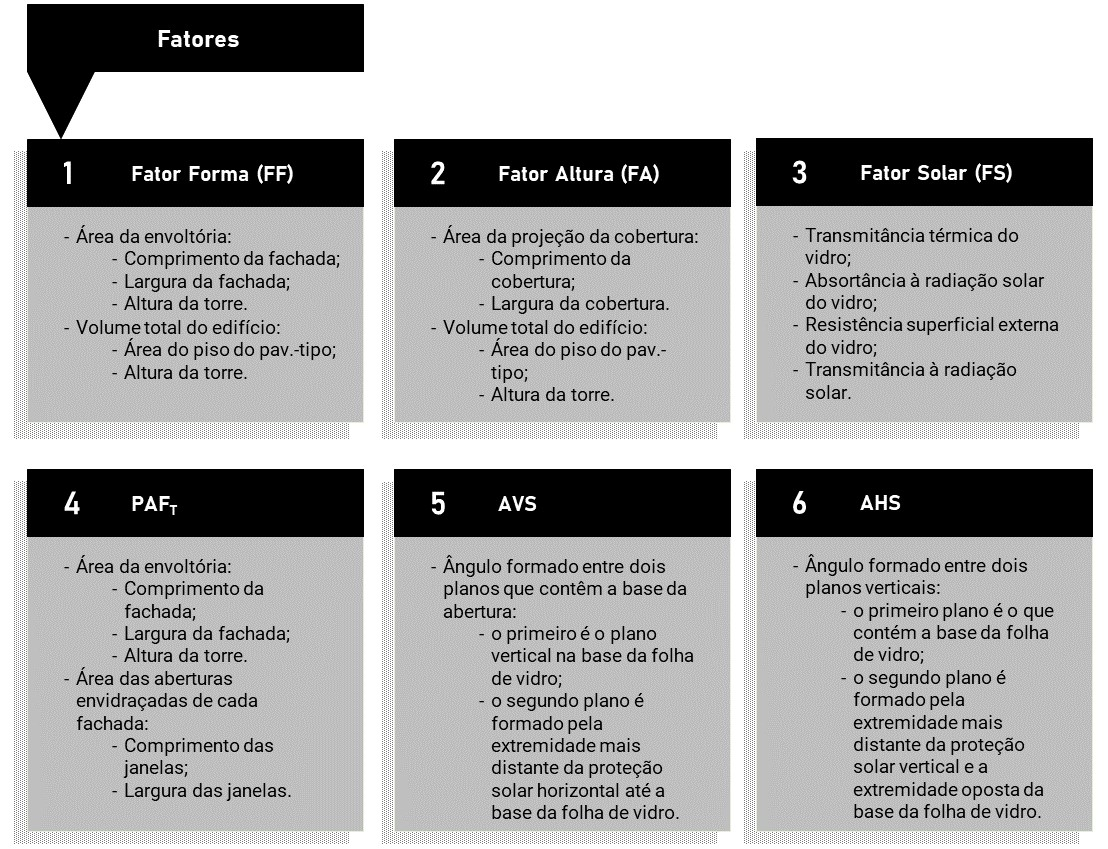
\includegraphics[width=0.9\textwidth]{figures/fig10_Fluxogramas-2.jpg}
        \begin{flushleft}
            \par \small Fonte: autor (2019).
        \end{flushleft}
        \label{fig:figura10}
    \end{figure}
    
Apresentados na Tabela 7 e exemplificado na Figura \ref{fig:figura11}, os atributos estudados foram Fator de 
Forma, FF, Fator Altura, FA, Percentual de Área de Abertura da Fachada Total, PAFT, Ângulo 
Vertical de Sombreamento, AVS, e Ângulo Horizontal de Sombreamento, AHS.
    \begin{figure}[ht]
        \centering
        \caption{\small Estrutura arquitetônica dos modelos genéricos.}
        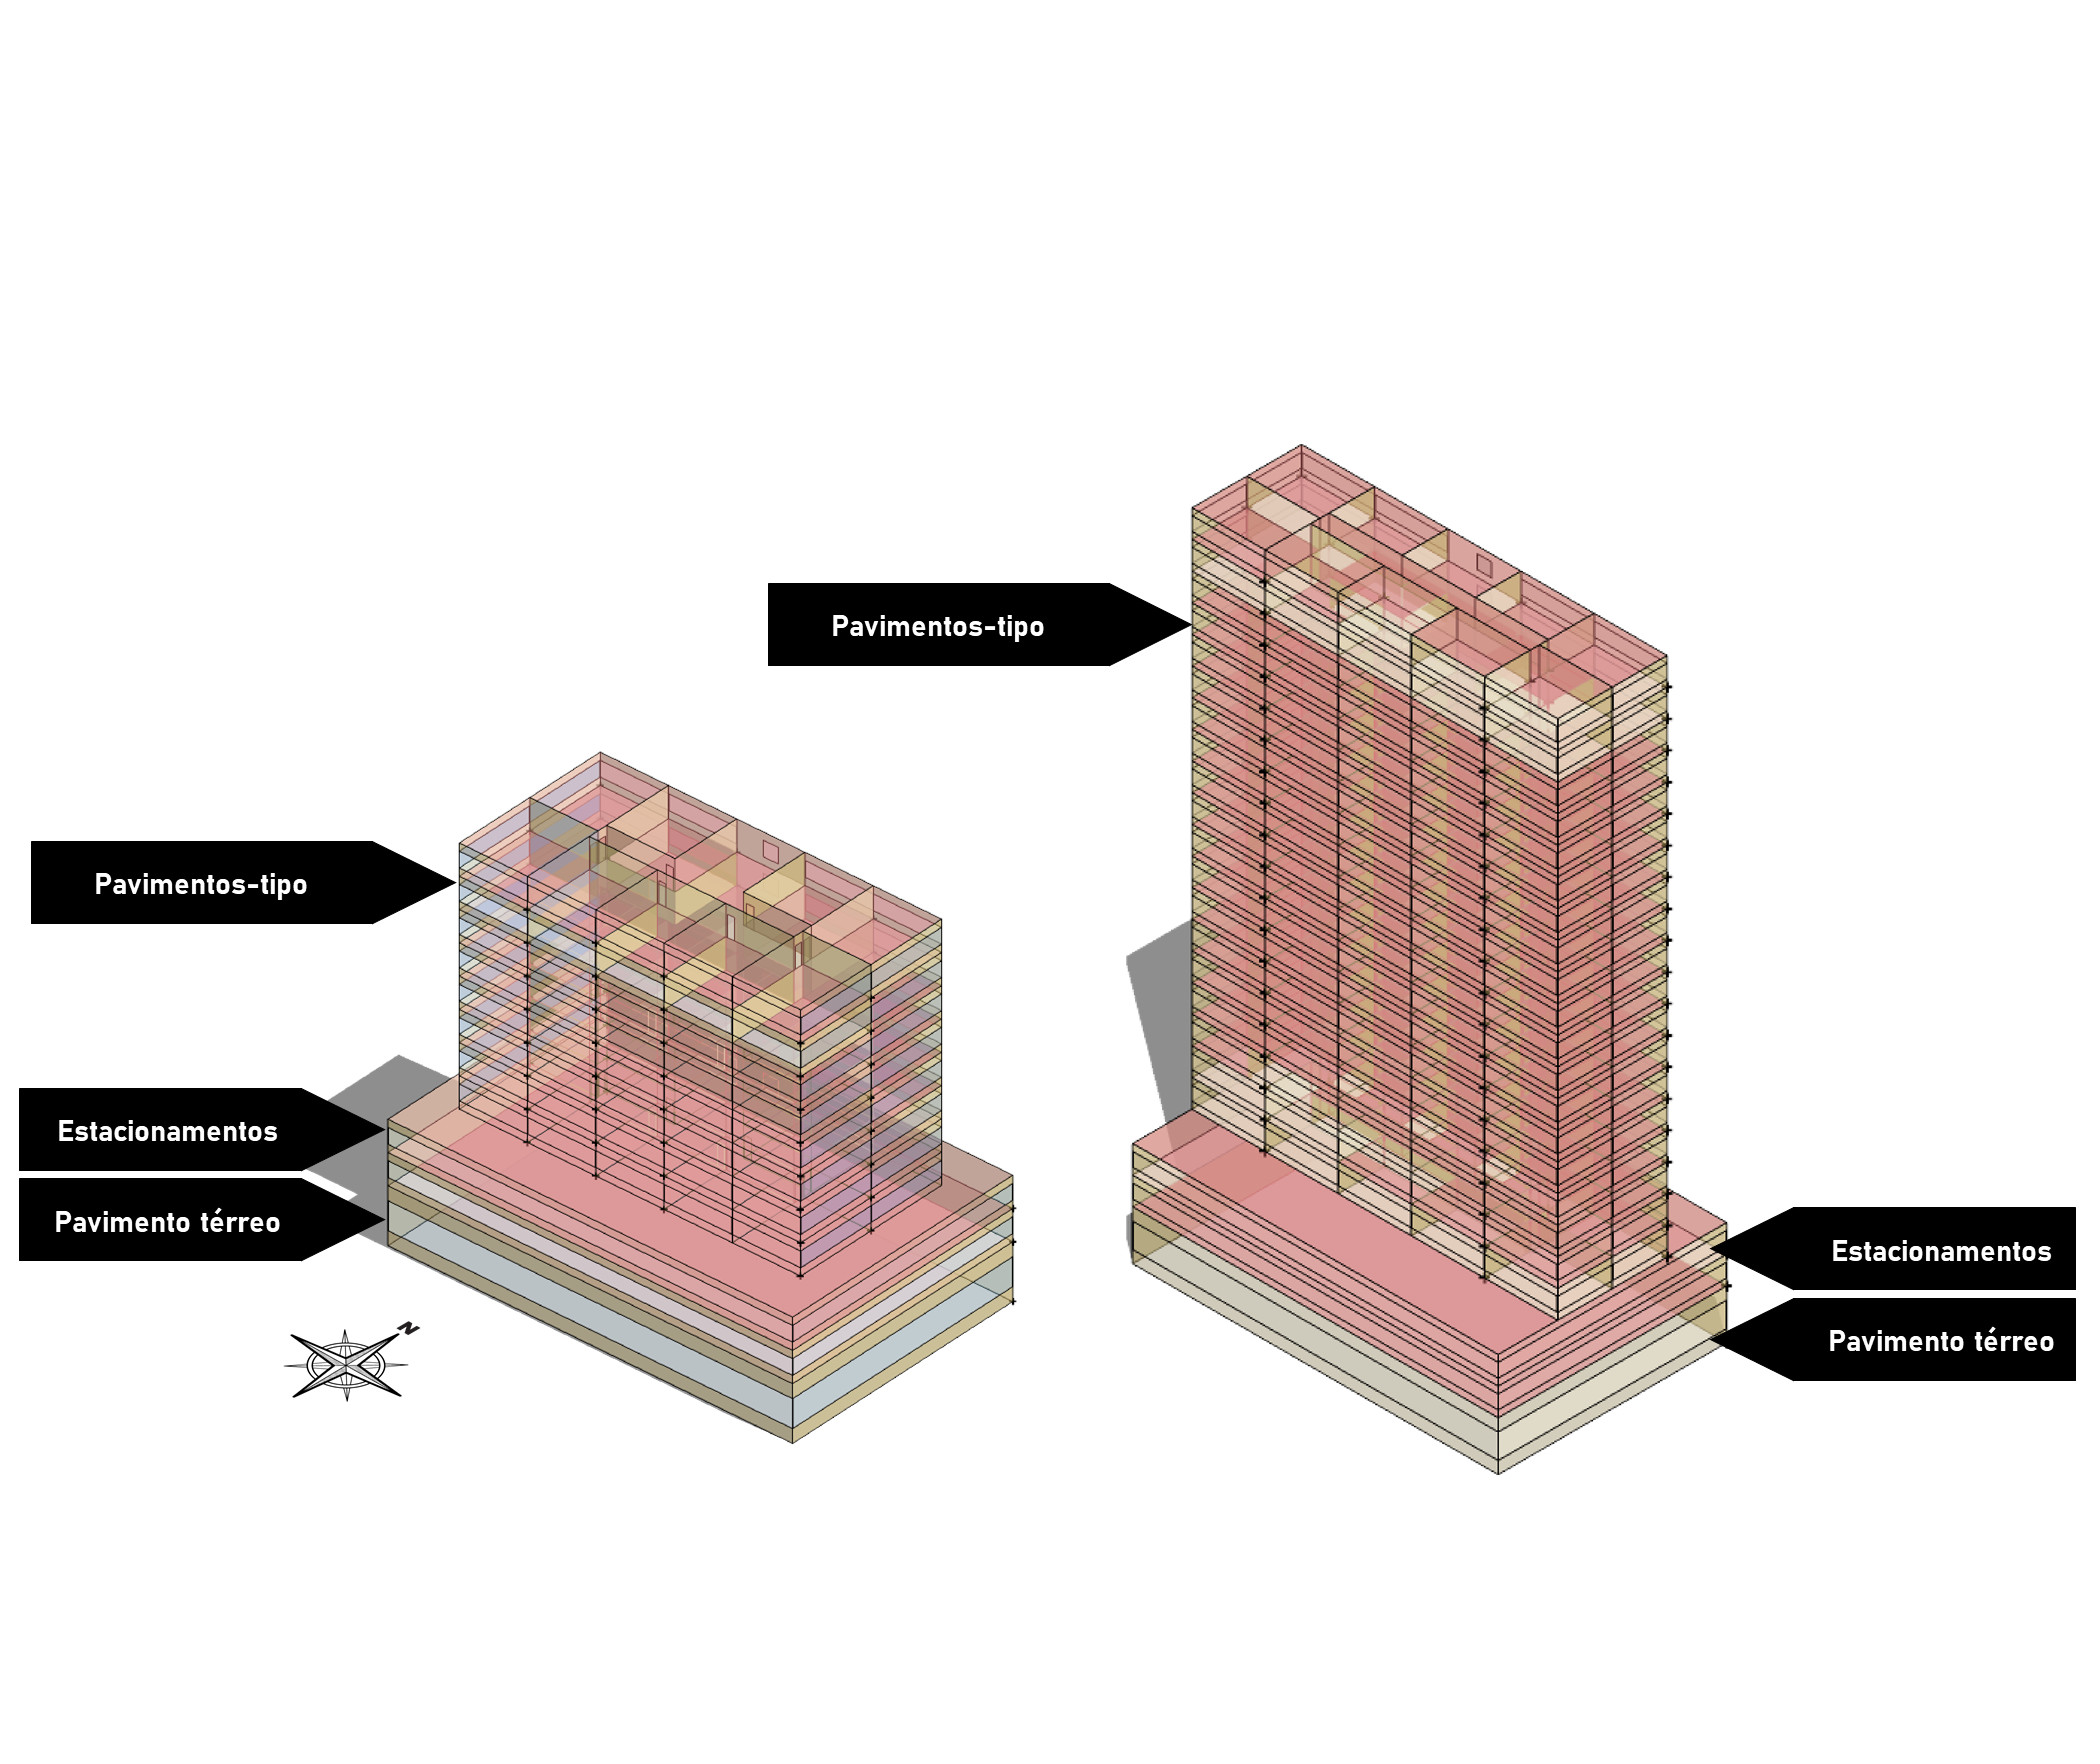
\includegraphics[width=0.9\textwidth]{figures/fig11_8-19-2pav.png}
        \begin{flushleft}
            \par \small Fonte: autor (2019).
        \end{flushleft}
        \label{fig:figura11}
    \end{figure}
